\begin{frame}
  \frametitle{\func{getWinninglay}}
  \input{tex/getwinningplay_tree}
\end{frame}

\begin{frame}
  \frametitle{Calcul de la compléxité}
  \newcommand{\enumeratenode}[1]{
  node{\scriptsize $\cdots #1 \cdots$} 
  edge from parent[draw=none]
}

\newcommand{\winnercomplexity}{\footnotesize $W(n)$}

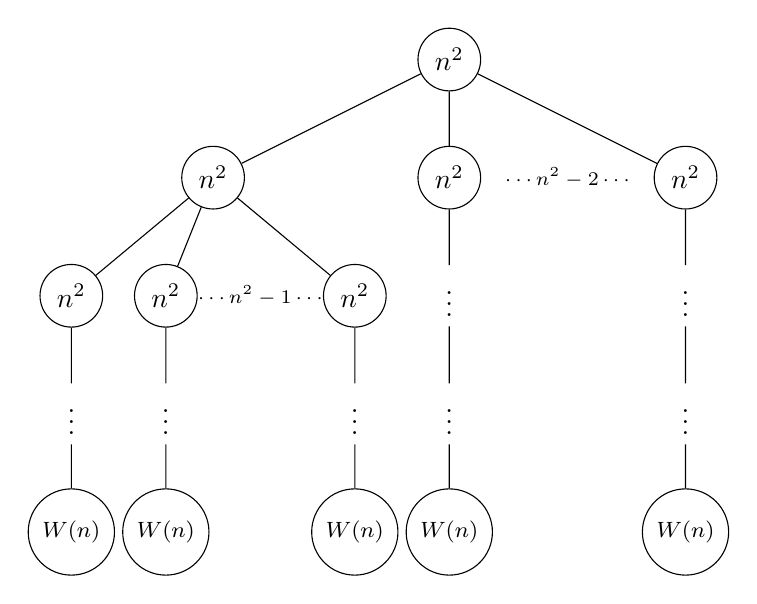
\begin{tikzpicture}

\tikzstyle{level 2}=[sibling distance=12mm]

\node[draw,circle]{$n^2$}
  child{node[draw,circle]{$n^2$}
    child{node[draw,circle]{$n^2$}
      child{node{$\vdots$}
        child{node[circle,draw]{\winnercomplexity}}
      }
    }
    child{node[draw,circle](g){$n^2$}
      child{node{$\vdots$}
        child{node[circle,draw]{\winnercomplexity}}
      }
    }
    child{\enumeratenode{n^2 - 1}}
    child{node[draw,circle](h){$n^2$}
      child{node{$\vdots$}
        child{node[circle,draw]{\winnercomplexity}}
      }
    }
  }
  child[missing]
  child{node[draw,circle](a){$n^2$}
    child{node{$\vdots$}
      child{node{$\vdots$}
        child{node[circle,draw]{\winnercomplexity}}
      }
    }
  }
  child{\enumeratenode{n^2 - 2}}
  child{node[draw,circle](b){$n^2$}
    child{node{$\vdots$}
      child{node{$\vdots$}
        child{node[circle,draw]{\winnercomplexity}}
      }
    }
  };

\end{tikzpicture}

\end{frame}

\begin{frame}
  \frametitle{Calcul de la compléxité d'un étage}
  Pour le $p$-ème étage.

  \pause

  $p$ coups à jouer parmis $n^2$ cases.

  \pause
  $\mathcal{A}^{n^2}_p$ noeuds
  \pause
  \begin{align*}
    E_p(n) &= \mathcal{A}^{n^2}_p n^2 \\
    \implies E_p(n)  &= \frac{(n^2)!}{(n^2 - p)!} n^2 \\
  \end{align*}
\end{frame}

\begin{frame}
  \frametitle{Calcul de la compléxité total}
  $n^2$ étages.
  \pause
  \[
    M(n) = \sum^{n^2}_{k = 1} E_p(n) + n^2! \; W(n)
  \]
  \pause
  \[
    M(n) = \sum^{n^2}_{k = 1} \left(\frac{(n^2)!}{(n^2 - p)!} n^2\right)
    + n^2! \; O\left(n^5\right)
  \]
  \pause
  \begin{align*}
    M(n) &= O\left(n^2! \; n^4\right) + n^2! \; O\left(n^5\right) \\
    \implies M(n) &= O\left(n^2! \;n^5\right)
  \end{align*}
\end{frame}
  
